\begin{frame}
\frametitle{Что такое ОС?}
\begin{figure}
    \hspace*{\fill}
    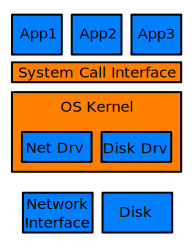
\includegraphics[height=.5\textheight]{os-outer-view}
    \hspace*{\fill}\hspace*{\fill}
\end{figure}
\end{frame}

\begin{frame}
\frametitle{Сервисы ОС}
\begin{itemize}
    \item<1-> Доступ к устройствам
    \begin{itemize}
        \item например, мышь или клавиатура
        \item часто через файловый интерфейс
    \end{itemize}
    \item<2-> Файловая система
    \begin{itemize}
        \item файлы и каталоги
    \end{itemize}
    \item<3-> Создание и взаимодействие процессов
    \begin{itemize}
        \item сигналы, каналы и другие
        \item сетевое взаимодействие
    \end{itemize}
\end{itemize}
\end{frame}

\begin{frame}
\frametitle{Компоненты ОС}
\begin{figure}
    \hspace*{\fill}
    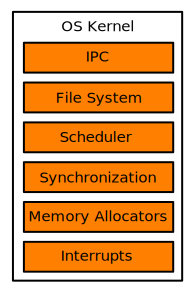
\includegraphics[height=.5\textheight]{os-inner-view}
    \hspace*{\fill}\hspace*{\fill}
\end{figure}
\end{frame}

